% ICLR full-width motivation figure; requires graphicx.
\begin{figure}[t]
  \centering
  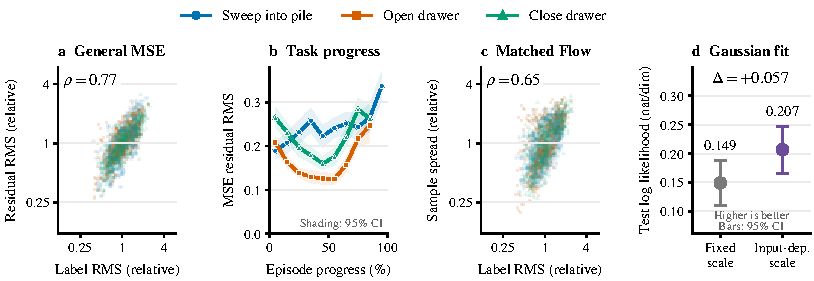
\includegraphics[width=\linewidth]{analysis/paper/widowx_heterogeneous_scale/fig_widowx_heterogeneous_scale.pdf}
  \caption{\textbf{General-MSE residuals and Flow spread on matched WidowX
  observations.} We freeze the general GR00T N1.7 MSE and Flow policies at
  20k training steps and evaluate both on the same 1,728 demonstration states
  from 144 BridgeData V2 episodes. Colors identify the three most frequent
  nonempty task instructions; all measurements use eight-step chunks of the
  six continuous action channels, excluding the gripper.
  \textbf{(a)} General-MSE residual RMS versus demonstration-label RMS.
  \textbf{(b)} Residual RMS over progress within each task; each point pools
  a 10\% progress interval, and shading denotes a 95\% episode-bootstrap
  confidence interval. The final seven frames are omitted to avoid padding.
  \textbf{(c)} Flow spread, measured as the RMS deviation of 16 samples from
  their mean, versus the same labels at exactly the same inputs as (a).
  Axes in (a) and (c) are normalized by task-wise geometric means; $\rho$
  measures within-task rank correlation.
  \textbf{(d)} Gaussian log likelihood with a fixed variance within each
  task or an input-dependent variance, keeping the MSE action prediction
  fixed. Points are means and bars are 95\% episode-bootstrap intervals;
  higher is better. Five-fold episode holdout applies to the variance fit;
  the frozen policies were trained on the demonstration dataset.}
  \label{fig:widowx-heterogeneous-scale}
\end{figure}
